%%%%%%%%%%%%%%%%%%%%%%%%%%%%%%%%%%%%%%%%%
% Journal Article
% LaTeX Template
% Version 1.3 (9/9/13)
%
% This template has been downloaded from:
% http://www.LaTeXTemplates.com
%
% Original author:
% Frits Wenneker (http://www.howtotex.com)
%
% License:
% CC BY-NC-SA 3.0 (http://creativecommons.org/licenses/by-nc-sa/3.0/)
%
%%%%%%%%%%%%%%%%%%%%%%%%%%%%%%%%%%%%%%%%%

%----------------------------------------------------------------------------------------
% PACKAGES AND OTHER DOCUMENT CONFIGURATIONS
%----------------------------------------------------------------------------------------

\documentclass[oneside, 11pt, a4paper]{article}
%\usepackage{polski}
\usepackage[english, polish]{babel}
\usepackage[utf8]{inputenc} 
\usepackage{cite}

\usepackage{graphicx}

\usepackage[T1]{fontenc} % Use 8-bit encoding that has 256 glyphs
\linespread{1.0} % Line spacing

\usepackage[top=3cm, bottom=3cm, left=2.5cm, right=2.5cm, columnsep=8mm]{geometry}

\usepackage{multicol} % Used for the two-column layout of the document
\usepackage[hang, small,labelfont=bf,up,textfont=it,up]{caption} % Custom captions under/above floats in tables or figures
\usepackage{booktabs} % Horizontal rules in tables
\usepackage{float} % Required for tables and figures in the multi-column environment

\usepackage{ragged2e} % better justification than a standard one

\usepackage{url}
\usepackage{breakurl}
\usepackage[hidelinks, breaklinks]{hyperref} % For hyperlinks in the PDF
\urlstyle{same}
\hypersetup{breaklinks=true}
\Urlmuskip=0mu plus 1mu\relax
\def\UrlBreaks{\do\/\do-}

\usepackage{paralist} % Used for the compactitem environment which makes bullet points with less space between them
\usepackage{amsmath}

\usepackage{titlesec} % Allows customization of titles
\usepackage[labelsep=period,font=small,format=plain,labelfont=bf,textfont=up]{caption}

% Ensure that the period is added after each section and subsection title. Adjust the spacing of section and
% subsection titles
\newcommand{\addperiod}[1]{#1.}
%\titleformat{command}[shape]{format}{label}{sep}{before-code}{after-code}
\titleformat{\section}[runin]{\bfseries\centering}{\thesection.}{3pt}{\addperiod} % Change the look of the section titles
\titleformat{\subsection}[runin]{\bfseries}{\thesubsection.}{3pt}{\addperiod} % Change the look of the section titles
\titlespacing*{\section}{0pt}{6pt}{3pt}[0pt]
\titlespacing*{\subsection}{0pt}{3pt}{3pt}[0pt]

\usepackage{textcomp}

\setlength{\parindent}{0.4cm}

 \setlength{\parskip}{0mm}
 \let\oldbibliography\thebibliography
\renewcommand{\thebibliography}[1]{\oldbibliography{#1}
\setlength{\itemsep}{0pt}} %Reducing spacing in the bibliography.
\renewcommand\refname{Bibliografia}

%----------------------------------------------------------------------------------------
% TITLE SECTION
%----------------------------------------------------------------------------------------

\title{\fontsize{14pt}{10pt}\vspace{3.55mm}\selectfont\textbf{Metody głębokiego uczenia w~rozpoznawaniu obrazów}} % Article title

\author{
{\fontsize{12pt}{1.2em}\selectfont Jacek Witkowski} \\
{\fontsize{11pt}{1.2em}\selectfont Wydział Elektroniki i Technik Informacyjnych, Politechnika Warszawska,}\\
{\fontsize{11pt}{1.2em}\selectfont ul.~Nowowiejska 15/19, 00-665 Warszawa}\\
{\fontsize{11pt}{1.2em}\selectfont \href{mailto:j.witkowski@stud.elka.pw.edu.pl}{j.witkowski@stud.elka.pw.edu.pl}} 
\date{}
}


%----------------------------------------------------------------------------------------
\frenchspacing
\begin{document}

\maketitle % Insert title

%----------------------------------------------------------------------------------------
% ARTICLE CONTENTS
%----------------------------------------------------------------------------------------

\begin{multicols}{2} % Two-column layout throughout the main article text

%\begin{abstract}
\section*{Streszczenie}

\textit{
W~artykule zwrócono uwagę na~dynamiczny rozwój Sztucznej~Inteligencji w~ostatnich czasach. Następnie objaśniono różnice pomiędzy uczeniem nadzorowanym i~nienadzorowanym oraz zaprezentowano przykładowe zastosowania Uczenia Maszynowego we~współczesnym świecie. Omówiono również temat sztucznych sieci neuronowych: ich~budowę oraz zasadę działania. Następnie wyjaśniono czym jest uczenie głębokie. Kolejno, zaprezentowano szczególny przypadek sieci neuronowej, jakim jest sieć splotowa. Wyjaśniono, w jaki sposób jest ona wykorzystywana do~rozpoznawania obiektów znajdujących się~na~obrazach. Zaznaczono również, że~zagadnienie to~jest tematem pracy magisterskiej autora artykułu.
}

\section{Motywacja}
Ostatnimi czasy Sztuczna Inteligencja jest wykorzystywana w~coraz większej liczbie obszarów. Zaczyna ona być obecna nawet w~urządzeniach codziennego użytku. Szybki rozwój Uczenia Maszynowego, czyli dziedziny zajmującej się badaniem Sztucznej Inteligencji, stał się~możliwy dzięki osiągnięciu znacznych mocy obliczeniowych komputerów. Pozwoliło to~na~stosowanie zaawansowanych algorytmów, które kiedyś były jedynie przedmiotem rozważań teoretycznych.

Biorąc pod~uwagę to,~że Sztuczna Inteligencja może być stosowana w~prawie każdej dziedzinie nauki, warto zgłębić wiedzę na~temat najnowszych osiągnięć związanych z~Uczeniem Maszynowym. W~przeciągu ostatnich 5~lat wyjątkowo szybko rozwijały się~algorytmy służące do~rozpoznawania obrazów. Prawdopodobnie było to spowodowane tym, że~jest to~obszar, w~którym można znaleźć wiele zastosowań dla~Sztucznej Inteligencji.

Jednym z~mechanizmów najczęściej wykorzystywanych do~rozpoznawania obrazów oraz materiałów wideo jest tzw.~sieć splotowa, która zostanie dokładniej omówiona w~dalszej części artykułu.

\section{Uczenie nadzorowane i nienadzorowane}
Mechanizmy Sztucznej Inteligencji można podzielić na:
\begin{compactitem}
	\item uczenie nadzorowane,
	\item uczenie nienadzorowane.
\end{compactitem}
\vspace{2mm}

\textbf{Uczenie nadzorowane} to~proces, w~którym wraz z~danymi wejściowymi sieci, dostarczamy do~uczonego mechanizmu również wynik spodziewany na~jego wyjściu. Wówczas celem uczenia jest minimalizacja różnicy pomiędzy danymi wygenerowanymi przez~mechanizm, a~danymi spodziewanymi.

W~\textbf{uczeniu nienadzorowanym} w~procesie uczenia dostarczane są~jedynie dane wejściowe (bez spodziewanego wyjścia, czyli tzw.~etykiet). Wówczas celem uczenia jest modelowanie danych wejściowych (a~dokładniej: rozkładu prawdopodobieństwa danych wejściowych). Przykładowo:~przy~uczeniu sieci neuronowej w~sposób nienadzorowany, jeśli będzie ona otrzymywała obrazki ludzkich twarzy, to~będzie w~stanie rozpoznawać często występujące zależności pomiędzy pikselami (np.:~krawędzie, nos, oczy, usta, jak również twarze).

Oba rodzaje uczenia mogą być łączone. W~ten sposób działa również mózg człowieka. By~zobrazować omawiane podejście, warto posłużyć się~przykładem. Wyobraźmy sobie, że~ktoś chce nas nauczyć rozpoznawać różne rodzaje jabłek. Najprostszym podejściem byłoby pokazywanie nam wielu jabłek wraz z~opisem wskazującym jakiego rodzaju jest każde z~nich. Byłoby to~jednak bardzo czasochłonne, gdyż~zaprezentowanie każdego jabłka wymagałoby przygotowania dla~niego odpowiedniego opisu. Łatwiejszym sposobem byłoby zamknięcie nas w~pokoju z~wieloma nieopisanymi jabłkami. Wówczas zaczęlibyśmy oglądać każde z~nich i~po~pewnym czasie zauważylibyśmy różne cechy powtarzające się~na~niektórych jabłkach (np.~podłużny kształt, czerwony kolor, zielony kolor, zielone plamki itp.). Po~wyjściu z~pokoju potrafilibyśmy identyfikować cechy występujące w~różnych grupach jabłek. Wiedza ta~pozwoliłaby nam na~nauczenie się~rozpoznawania różnych gatunków na~podstawie mniejszej liczby opisanych przykładów niż~przy~podejściu naiwnym, gdzie od~początku stosowane jest uczenie nadzorowane.

\section{Przykłady zastosowań}
\subsection{Ocena atrakcyjności zdjęć}
By~lepiej zrozumieć, jakie możliwości otwiera przed~nami obecny rozwój Uczenia Maszynowego, warto poznać zastosowania, jakie~znajduje ta~dziedzina już teraz. Jednym z~nich jest zastosowanie Głębokiej Splotowej Sieci Neuronowej (\textit{\mbox{ang.~Convolutional} Neural Network, CNN}) do~oceniania atrakcyjności zdjęć ,,selfie'' \cite{SelfieCNN}. W~omawianym projekcie autor:
\begin{compactenum}
	\item Zgromadził zdjęcia, które oznaczone były hasz-tagiem ,,selfie'' (znalazł około 5 milionów takich zdjęć).
	\item Przy~użyciu mechanizmu rozpoznającego twarze na~obrazkach wybrał tylko te~zdjęcia, na~których obecna była przynajmniej jedna twarz (zostało około 2~milionów zdjęć).
	\item Posortował fotografie względem liczby użytkowników obserwujących autora danego zdjęcia.
	\item Podzielił posortowaną listę fotografii na~grupy po~100 zdjęć (każda grupa dzięki temu zawierała zdjęcia o~podobnej liczbie obserwujących danego użytkownika).
	\item W~obrębie każdej grupy, utworzył ranking zdjęć na~podstawie ich liczby polubień. Górna połowa zdjęć była uznawana za~zdjęcia dobre, a~dolna~-~za~złe.
	\item Trenował sieć neuronową milionem zdjęć dobrych oraz milionem zdjęć złych. Dzięki temu mechanizm nauczył się~odróżniać oba typy zdjęć.
\end{compactenum}
Tak~utworzona Splotowa Sieć Neuronowa była w~stanie ocenić prawdopodobieństwo, że~dane ,,selfie'' jest atrakcyjne (im~wynik na~wyjściu sieci był wyższy, tym~zdjęcie było lepiej oceniane).

\subsection{Image Super Resolution}
Innym przykładem zastosowania Uczenia Maszynowego jest projekt Image Super Resolution \cite{SuperResolution}. W~swojej aplikacji autor użył Sztucznej Inteligencji w~celu czterokrotnego powiększania obrazków: z~rozmiaru 16x16 pikseli do~64x64 piksele. Porównanie wyników działania sieci neuronowej oraz interpolacji bikubicznej (standardowej metody stosowanej do~powiększania obrazów w~programach graficznych) zostały przedstawione na~rysunku \ref{fig:superresolution}.
Architektura zastosowana w~projekcie to~DCGAN (\textit{ang. Deep Convolutional Generative Adversarial Network}, Głęboka Generatywna Antagonistyczna Sieć Splotowa \cite{DBLP:journals/corr/RadfordMC15}). Wykorzystuje ona uczenie nienadzorowane.
W~uproszczeniu: autor mechanizmu w~procesie uczenia używał obrazków przedstawiających twarze. Sieć nauczyła się~wówczas jakie są~najczęstsze zależności pomiędzy pikselami występujące w~tych obrazkach, a~więc mogła również generować twarze.
Etap ten był uczeniem nienadzorowanym. Następnie autor zastosował kolejny uczenie nadzorowane, w~którym jako funkcję błędu wykorzystał odległość L1 pomiędzy wynikiem powiększania obrazka przez~sieć, a~oryginalnym obrazkiem o~rozmiarze 64x64 piksele. Odległość L1 (inaczej odległość Manhattan) jest zdefiniowana jako suma różnic odpowiadających sobie współrzędnych dwóch wektorów, tj.~$\sum\limits_{i=0}^n (x_i - y_i)$, gdzie $n$ to~liczba współrzędnych (w~tym wypadku: liczba pikseli pomnożona przez~liczbę kanałów, która dla~obrazu kolorowego jest równa 3), a~$x$ i~$y$ to~porównywane obrazki.

\begin{figure}[H]
	\centering
	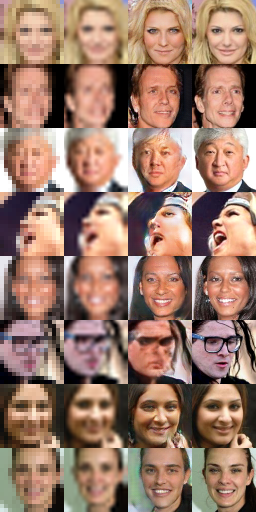
\includegraphics[width=0.9\linewidth, keepaspectratio]{img/srez_sample_output.png}
	\vspace{-2mm}
	\caption{Powiększanie obrazków (pierwsza kolumna zawiera powiększany obraz, druga~-~obraz powiększony poprzez zastosowanie interpolacji bikubicznej, trzecia~-~obraz powiększony przez~sieć splotową, czwarta~-~oryginalny obraz 64x64 piksele).}
	\label{fig:superresolution}
\end{figure}
\vspace{-0.3cm}
\subsection{AlphaGO}
Do~bardziej zaawansowanych Sztucznych Inteligencji należy projekt ,,AlphaGo''\cite{AlphaGO} stworzony przez~firmę Google~DeepMind. Owa~Sztuczna Inteligencja nauczyła się~grać w~starochińską grę planszową~-~Go. Mechanizm wyróżnia to,~że~może być wykorzystany do~różnych celów (np.~może nauczyć się~grać w~inne gry) i~nie~był tworzony pod~z~góry określone zastosowanie, w~przeciwieństwie do~mechanizmów takich jak: IBM~Watson czy~IBM~Deep~Blue. Silnik stworzony przez~firmę~---~DeepMind~---~jako~dane wejściowe przyjmuje obraz w~postaci mapy bitowej, a~następnie do~jego przetwarzania wykorzystuje głębokie splotowe sieci neuronowe (opisane w~dalszej części artykułu) oraz Q-learning (szczególny rodzaj uczenia ze~wzmocnieniem).

Program AlphaGo jest przełomowy również pod~innym względem: jest pierwszą Sztuczną Inteligencją, która~pokonała profesjonalnego gracza w~Go \cite{FanHuiGO} na~pełnowymiarowej planszy (19x19) bez~zastosowania tzw.~handicapu. Pojedynek odbył się~w~październiku~2015 roku. Niedługo potem, w~marcu~2016 roku, AlphaGo zdołał pokonać, 18-krotnego i~również ówczesnego mistrza świata w~grę~Go \cite{LeeSedolGO}.

Tym~samym ostatnia z~popularnych gier planszowych straciła mistrza ludzkiego na~rzecz programu komputerowego (podobnie jak~wcześniej warcaby\cite{checkersSolved} czy~szachy\cite{newborn1997kasparov}).

\section{Sieci neuronowe}
Jednym z~mechanizmów, który jest najczęściej wykorzystywany do~implementacji Sztucznej Inteligencji, jest sztuczna sieć neuronowa. Jest ona~inspirowana sieciami neuronowymi występującymi w~biologii (np.~w~ludzkim organizmie, w~szczególności: w~mózgu). Na~strukturę sieci składają się~pojedyncze połączone ze~sobą elementy, zwane neuronami. Budowa neuronu została przedstawiona na~rysunku \ref{fig:hebb-neuron}.
\begin{figure}[H]
	\centering
	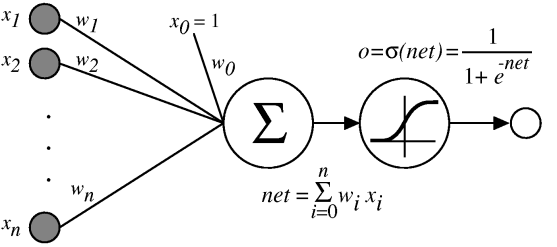
\includegraphics[width=0.9\linewidth, keepaspectratio]{img/sigmoid-neuron.png}
	\vspace{-2mm}
	\caption{Neuron Hebba.}
	\label{fig:hebb-neuron}
\end{figure}

Neurony najczęściej łączone są~w~tzw.~sieci warstwowe. Przykładowa sieć warstwowa została zaprezentowana na~rysunku \ref{fig:feed-forward-net}. Jeśli liczba warstw występujących w~danej sieci jest dostatecznie duża (zazwyczaj: około 10~warstw lub~więcej), sieć określana jest jako~głęboka.

Algorytm, który pozwala otrzymać wartość wyjściową dla~neuronu, przedstawia się~następująco:
\begin{compactenum}
	\item Pobierz dane wejściowe, które są~wektorem: $\overline{X}=[x_1, x_2, ..., x_n]$.
	\item Pomnóż każdą współrzędną wektora wejściowego przez~odpowiadającą mu~wagę (określaną w~procesie uczenia sieci) i~zsumuj ze~sobą otrzymane wartości: $net = \sum\limits_{i=0}^{n} w_i x_i$.
	\item Do~otrzymanego wyniku dodaj czynnik $b$ zwany przesunięciem (\textit{ang.~bias}): $net := net + b$.
	\item Otrzymaną sumę poddaj działaniu funkcji $\sigma$ zwanej funkcją aktywacji: \mbox{$o=\sigma(net)$}. Wynik tej operacji jest wartością wyjściową neuronu.
\end{compactenum}
\begin{figure}[H]
	\centering
	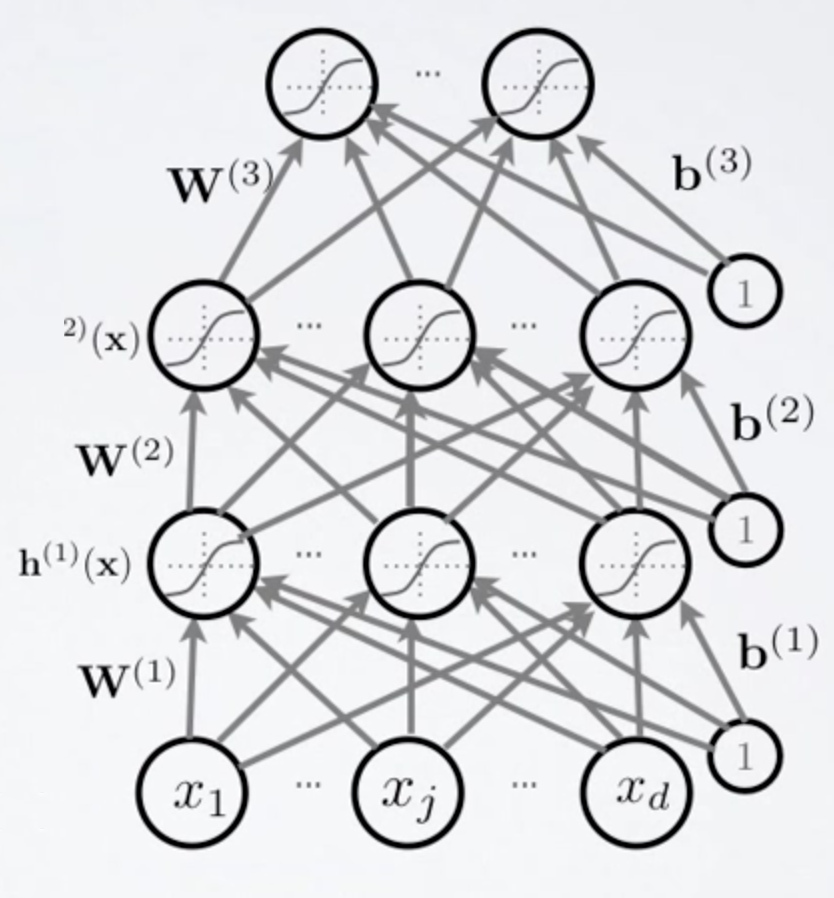
\includegraphics[width=\linewidth]{img/feed_forward_neural_network.png}
	\vspace{-8mm}
	\caption{Warstwowa sieć neuronowa typu Feed-Forward. Źródło: \cite{feed-forward-net-source}}
	\label{fig:feed-forward-net}
\end{figure}
\vspace{-5mm}
\section{Splotowe sieci neuronowe}
Szczególnym przypadkiem sieci neuronowych są~sieci splotowe. Wykorzystują one operację splotu w~postaci dyskretnej:
\begin{align*}
(f \ast g)[n] = \sum\limits_{m=-\infty}^{+\infty}f[m]g[n-m]\\
=\sum\limits_{m=-\infty}^{+\infty}f[n-m]g[m]
\end{align*}

Dzięki stosowaniu różnych masek (funkcji splatanych z~przetwarzanym sygnałem, np.~obrazem) w~filtrach splotowych można uzyskiwać różne efekty. Istnieje wiele zdefiniowanych funkcji tego typu, które służą m.in.~do:
\begin{compactitem}
	\item redukcji szumów,
	\item wyostrzania,
	\item wykrywania krawędzi.
\end{compactitem}

Sieci splotowe wykorzystują to,~że~odpowiednio dobierając wartości maski, można uzyskiwać bardzo różne efekty. Jednak maska zamiast przyjmować z~góry zadane wartości (tak~jak~w~standardowych filtrach splotowych), otrzymuje je~w~procesie uczenia.

Standardowym zadaniem, do~którego wykorzystywane są~splotowe sieci neuronowe, jest identyfikacja obiektu obecnego na~zdjęciu. Algorytm przetwarzania obrazu dzieli się~na~etapy:
\begin{compactenum}
	\item Splot~-~zastosowanie $n$~różnych filtrów splotowych, wynikiem czego jest $n$~obrazków zwanych mapami cech.
	\item Normalizacja (krok opcjonalny, mający na~celu taką zmianę danych, która poprawi jakość uczenia sieci). Krok ten wyjaśniono w~dalszej części artykułu).
	\item Próbkowanie (zmniejszenie rozmiarów powstałych map cech, m.in.~w~celu redukcji rozmiaru przetwarzanych danych).
	\item Powtórzenie kroków 1-3 wiele razy (liczba powtórzeń jest zależna od~liczby warstw w~sieci).
	\item Przekazanie powstałych map cech do~warstwy neuronów w~pełni połączonej (każdy piksel trafia do~wszystkich neuronów tej warstwy sieci).
	\item Zastosowanie kolejnych warstw w~pełni połączonych (zazwyczaj w~sieci stosuje się~jedną lub~dwie takie warstwy).
	Ostatnia z~tych warstw ma~za~zadanie przedstawić na~swoim wyjściu prawdopodobieństwa występowania różnych etykiet (np.~kot:~50\%, pies:~20\%, samochód:~5\%, ...)
\end{compactenum}

Drugi krok, czyli normalizacja, jest krokiem, w~którym zawierają się~różne operacje mające na~celu taką zmianę danych, by~proces uczenia uległ poprawie (np.~szybsze uczenie sieci, lepsza jakość klasyfikacji w~sieci). Jest to~zagadnienie bardzo obszerne i~nie~jest omawiane w~tym~artykule.

Splotowe sieci neuronowe szczególnie często są~wykorzystywane do~przetwarzania obrazów i~filmów.
Jest to~spowodowane tym, że~mogą one operować na~danych wielowymiarowych (tj.~obrazach czy filmach), a~przy tym potrafią znajdywać lokalne cechy występujące w~sygnale (np.~człowiek może pojawiać się~w~różnych miejscach na~zdjęciu, a~sieć zawsze będzie w~stanie określić, że~fotografia przedstawia człowieka).

\section{Podsumowanie}
Z~powodu gwałtownego wzrostu mocy obliczeniowej w~ciągu ostatnich 10~lat znacząco zwiększyły się~możliwości mechanizmów wykorzystujących Sztuczną Inteligencję. Wciąż rośnie liczba obszarów, w~których Uczenie Maszynowe znajduje zastosowania: od~automatycznych tłumaczeń tekstów, poprzez samosterujące się~pojazdy, gry planszowe oraz komputerowe, medycynę, aż~do~wszelkiego rodzaju zagadnień związanych z~obróbką obrazów czy~materiałów wideo. Ostatnie~z~wymienionych zastosowań (przetwarzanie materiałów graficznych oraz audio-wizualnych) szczególnie często wykorzystuje głębokie sieci splotowe, czyli specyficzny rodzaj sieci neuronowych, składających się~z~wielu warstw, wykorzystujących filtry splotowe do~osiągania założonych celów (np.~identyfikacji obiektów znajdujących się~na~zdjęciach czy~wręcz tworzenia opisów tych obrazów w~języku naturalnym).

Z~powodu mnogości istniejących zastosowań dla~sieci splotowych oraz prawdopodobnie wielu dziedzin wciąż czekających na~wsparcie ze~strony mechanizmów tego rodzaju, warto zgłębić tę~szczególną gałąź Uczenia Maszynowego. Zadaniem referencyjnym, które jest często wykorzystywane do~badań nad~sieciami splotowymi jest identyfikacja przedmiotów przedstawionych na~obrazkach. Istnieją również bazy opisanych etykietami zdjęć takie jak CIFAR-10 i CIFAR-100\cite{cifar10and100} czy~ImageNet\cite{imagenet}, które mogą posłużyć jako~zbiór danych treningowych i~testowych. 

W~ramach swojej pracy magisterskiej stworzyłem głęboką splotową sieć neuronową realizującą wymienione zadanie referencyjne. Ze~względu na~niewielką moc obliczeniową urządzeń, z~których mogłem korzystać, posłużyłem się~bazą CIFAR-10. Pozwoliło to~zbadać wpływ różnych parametrów sieci na~jakość uczenia i~klasyfikacji. Badano między innymi zachowanie sieci z~różnymi algorytmami normalizacji, różnymi modelami neuronu oraz przedstawiono proces ulepszania sieci poprzez zmianę jej architektury. Wiedza ta pozwala konstruowanie większych sieci, w~celu realizacji bardziej złożonych obliczeniowo zadań rozpoznawania obrazów.

\vfill
%----------------------------------------------------------------------------------------
% REFERENCE LIST
%----------------------------------------------------------------------------------------
\raggedright


\bibliography{bibliography}{}
\bibliographystyle{unsrt}

%----------------------------------------------------------------------------------------

\end{multicols}

\end{document}